

In the first section of this chapter, any difficulties faced while installing the software on different systems are described. Then the first performance experiments are presented, followed by profiling of the code with two different profilers. Finally, some elementary efforts to optimise the performance, based on the conclusions reached from the analysis, are presented.



\section{Installation adventure}

        The procedure described on sections \ref{nninstall} and \ref{nnuse} was followed in order to install and execute the software on the three computing systems mentioned in section \ref{ch:nnwhere}. Although, the installation, for the most part, was smooth, a small number of errors had to be dealt with.
        
        \begin{itemize}
            \item[]\textbf{During installation:}
            \item An old version of SciPy, a scientific python package, was being installed by default. This was causing conflicting dependencies with the other packages and the installation would fail. \\
            To fix that, the installation script was changed so that the latest version of SciPy is being used.
            \item Joblib, a module that aids parallelising loops in Python, was not being installed by the script but was required.\\
            As a fix, the joblib module was added to the installation script.
            \item[]\textbf{On execution:}
            \item The interpreter would complain about a variable that was out of scope and quit.\\
            The bug was fixed by defining the variable in a more appropriate place.
            \item Midway through the project, after cloning the latest commit from the repository, the software stopped working. The reason was that the format of the input file was changed. Thus the existing input file that was supplied to the student became obsolete.\\
            A new input file was provided by the physics department. Also, a new branch to work on was created in the repository to be immune to future software commits by the developing team.  
        \end{itemize}
        

\section{Computing Systems Used}\label{ch:nnwhere}
As the neural network can be run on either CPU or GPU machines, two main systems were chosen, Cirrus and Jade. Also, for quick GPU runs a small system called deeplearn was used.
    \subsection{Cirrus}
    Cirrus was the main system used for CPU performance measurements of the neural network for the same reasons it was chosen for FastJet.
        \subsubsection{Hardware}
        The hardware of Cirrus is discussed in section \ref{ch:cirrus}. 

    \subsection{Jade}
    Jade is the largest GPU facility in the UK. Since access to it was granted for the dissertation, it was used for the GPU performance measurements of the neural network. Being a new system to the student, it took some time to gain familiarity. As the project progressed though, the focus was more and more towards GPU performance. Consequently, most of the results presented in this chapter, come from Jade. 
        \subsubsection{Hardware}
        Jade\cite{jade1} is a UK academic Tier-2 resource and consists of 22 nodes, each containing 8 NVIDIA Tesla P100 GPU cards, linked by NVIDIA's NV link interconnect.  
    
        \subsubsection{Running on the back-end}
        Submitting a job to the back-end of JADE would result to an error about not having permission to do so. A claim was submitted to the technical support team and a few days later the appropriate permissions were granted and the issue was resolved.
        
        The JADE submission script allows the user to chose the desired number of GPU cards to be reserved. Initially, the same number of cards that would be used by the software were also reserved. It was noticed that the timing results were not consistent. This was attributed to the fact that the CPU inside a node cannot be reserved, and could potentially be shared with other users. 
        
        As a solution, every submission script was requested for 8 GPU cards (a whole node), to make sure that the CPU was also reserved. Jobs then, waited in the queue a much longer amount of time, but the timing results were consistent. 
        
    \subsection{Deeplearn}
    The JADE GPU facility is generally very busy. Requesting a whole node for every experiment run would result in wasting a lot of time. To account for that and any time period that Jade would be unavailable, a small system, deeplearn, monitored by EPCC was used. 
    
    Although no results presented in this chapter, originated from deeplearn, the system was extremely helpful for running quick experiments, that did not necessarily have to be ran on Jade. 

    \subsubsection{Hardware}
        Deeplearn consists of an Intel Quad Core 2.40GHz CPU, 8GB of RAM and an NVIDIA GeForce GTX TITAN X graphics card.
        
\section{Does it run on GPU?}
On JADE and Deeplearn, it was not immediately clear that after adding the \verb|--|gpu argument, the training was performed on the GPU cards. Other than the performance being better than from using the \verb|--|cpu argument, nothing else indicated that the training took place on the GPU card.

Since the neural network can output a Tensorboard log file, that file would be use to get an answer. Tensorboard requres port forwarding to visualise the results, which is not allowed in Jade; the firewall seems to be blocking port forwarding. As a workaround, the tensorboard log file was copied to the student's laptop and then visualised. 

After that, Tensorboard worked and provided insightful information regarding the model. Figure \ref{fig:tensorboard2} is a visualisation of the classifier model; the combined model was to complex to present. Even though Tensorboard's result was informational, it didn't succeed in the providing an answer to what whether the GPU cards are being used. The output would read "unknown device". Thus an alternative was sought.

\begin{figure}[H]
    \centering
    \includegraphics[width=\linewidth]{images/tensorboardgraph1.jpeg}
    \caption{this is wrong. fix me}
    \label{fig:tensorboard2}
\end{figure}


To determine if the GPU cards are being utilised, another strategy was followed. The the neural netwrork was being executed in the background, and the command nvidia-smi was called. This command provides information on the GPU cards existing on the system, like their utilisation, the processes currently using them, their temperature, and more. As can be seen from figure \ref{fig:smi}, the background python code previously executed is using the GPU card, and the utilisation is 25\%. At that point it became clear that the neura network was utilising the GPU cards.
        
        \begin{figure}[H]
            \centering
            \includegraphics[width=\linewidth]{images/smi2.jpg}
            \caption{fix me: this is smi}
            \label{fig:smi}
        \end{figure}


The reasons for the low utilisation of the GPU cards are discussed further along the way.

\section{Measuring performance}
At that point of the dissertation, the neural network was installed and running on both big systems. It was time for some performance timings; but first the analysis framework should be set up.

\subsection{Performance analysis framework}
All the performance measures presented in this chapter, were run on the back-end of Cirrus if the they were ran on CPU and on the back-end of Jade if they were ran on GPU. 

Unless stated otherwise, timings represent the total run-time for the neural network to trai; this includes the classifier and the combined model. Every measurement presented in this report is the average of 3 runs. 

\subsection{First timing results}
Figure \ref{fig:nn_timings} shows the performance of the neural network on a single Cirrus node (36 CPU cores), and different number of GPU cards from Jade.

Interestingly but not unexpectedly, the performance of the neural network does not improve when more GPU cards are used. If one GPU card is underutilised, how will adding more cards aid performance?


\begin{figure}[H]
    \centering
    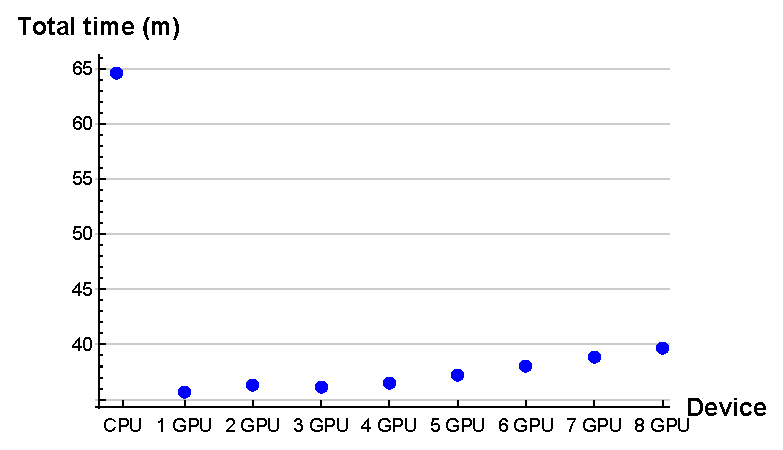
\includegraphics[width=\linewidth]{images/nnperf.eps}
    \caption{Caption:fix me}
    \label{fig:nn_timings}
\end{figure}
 
 
 \section{Profiling}
 \subsection{Vtune Amplifier for CPU profiling}
VTune Aplifier, proved to be a good ally in the performance analysis of FastJet. That was the reason, it was initially used to profile the neural network on Cirrus.

The process was rather trickier this time, as the code is written in python. Python makes use of a runtime interpreter instead of compiling. As a result, there was no binary file of the neural network to select as the executable. 

In order to profile, Python's executable file was selected as the binary to be profiled, and the neural network code was passed as an argument (figure \ref{fig:vtunenn1}).  

\begin{figure}[H]
    \centering
    \includegraphics[width=\linewidth]{images/vtunenn.JPG}
    \caption{Caption: fix me}
    \label{fig:vtunenn1}
\end{figure}

This method, succeeded in profiling the code, but the results were in assembly language. As a result, it was hard to reach any conclusions. The physics department was not particularly interested in performance analysis on CPU, thus the effort to profile the neural network on Cirrus was stopped there.

 
 \subsection{NVIDIA Visual Profiler for GPU profiling}
 To profile the neural network on JADE's GPU cards, NVIDIA Visual Profiler (nvprof), that is included with Cuda 9, was used. It was selected because nvprof specialises on the profiling of CUDA applications which is what is going on under the hood of the neural network.
 
 To profile the code on Jade and analyse the results on the students laptop, the instructions for remote profiling in the official documentation\cite{nvprof} were followed. This profiling process included two phases. The first one involved collecting a timeline of the application executing on the remote system, with the least possible intrusion by the profiler. It can be performed with the command 
 \begin{lstlisting}[language=bash]
nvprof --export-profile timeline.prof <app> <app args> \end{lstlisting}

Having done that, the next stage was to collect metrics for the kernels in the application.  This was much more intrusive that the previous phase, and significantly changed the overall performance because all kernel executions were serialised on the GPU. The command for it is
 \begin{lstlisting}[language=bash]
nvprof --metrics achieved_occupancy,executed_ipc -o metrics.prof 
    <app> <app args>\end{lstlisting}

For the second part of the profiling to finish in a reasonable amount of time, the number of epochs was set to 1 and only the classifier was trained. The output files from timeline and metrics were copied locally and opened with nvidia visual profiler. The profiler automatically merges the two results to get an accurate picture of the applications behaviour.

\begin{figure}[H]
    \centering
    \includegraphics[width=\linewidth]{images/nv13.jpeg}
    \caption{Caption: fix me}
    \label{fig:nvprof1}
\end{figure}

\begin{figure}[H]
    \centering
    \includegraphics[width=\linewidth]{images/nvwarning.jpeg}
    \caption{Caption: fix me2}
    \label{fig:nvprof2}
\end{figure}



Figure \ref{fig:nvprof1} shows the memory copies from Host (CPU) to the Device (GPU) and vice-versa, and the compute time for 2 representative seconds during the training. It can be seen that the memory copies to the Device are very often but Kernels quickly run out of work. The result of the guided analysis is shown in figure \ref{fig:nvprof2}.   

\textbf{(to do) Understand why 4/8 GPU were slower that one}

 
\section{Attempts made to improve performance}

 \subsection{Optimising data copying by hand}
 One of the goals set at the start of this dissertation was to improve the way data are being fed to the GPU cards. This is currently implemented by Keras calls, but there exists an old commit in the repository with a working simple parallelisation attempt. The plan was to retrieve it, revise it to work with any changes that took place in the meantime, and improve it.
 
That goal was left out for a number of reason. First of all, the commit is pretty old. Thus, a considerable amount of work-time would have to be put solely to make it work with the current state of the software. That is without even considering the time to improve it. Also, following discussions with the developing team, the simplicity and support offered by Keras implementation was preferred to a possible performance gain.

From that point onwards, the attempted optimisations were through Keras.  

\subsection{Tuning the batch size}
To address the under-utilisation of the GPU cards, different values of the bath size were tested to see how this affects performance. The speculation was that, bigger batch sizes would feed the Kernels with more work to do, maybe enough to work until the next batch of data comes.

Figure \ref{fig:batchsize1} show the result. For batch size values smaller than $2^9$ samples, the run-time was more than 10 hours and is not included, while for sizes bigger than $2^{17}$ samples, data would not fit in the memory of the GPU cards. The default value for the batch size is $2^{13}$ samples.

The bigger the batch size, the better the performance. Figure \ref{fig:batchsize2} shows the speed-up curve for different batch sizes. Got a 4x speedup.

It was noticed that altering the batch size affects also the training accuracy of the neural network. The model is less efficient when a bigger batch-size is used. Was the speed-up gained from altering the batch size in vain?


\subsection{Setting a stopping criterion} 
To investigate the relation between the batch size and the training accuracy of the neural network, a stopping criterion was set, instead of the constant 200 epochs. This way, the training would stop once a specific acuracy was reached, an the different batch sized could be compared  on equal terms.

KERAS provides a way to set a stopping criterion, through a function. The arguments of this function are:
\begin{itemize}
    \item \textbf{min\_delta:} minimum change of the loss function to qualify as an improvement.
    \item \textbf{patience:} number of epochs with no improvement after which training will be stopped.
    \item \textbf{baseline:} Baseline value for the monitored quantity to reach. Training will stop if the model doesn't show improvement over the baseline.  
\end{itemize}

Following discussions with the developing team, setting a hard threshold where the training would stop was the best solution, to compare the different batch sizes between them. Thus, baseline value was set to !!!!, patience to zero. 


The stopping criterion was only implemented on the classifier training. That is because, on the adversarial part of the neural network, the two networks are constantly antagonising each other and improving. The way that the combined model's accuracy is improving is not as straightforward.


Figure \ref{fig:criterion1} shows the number of epochs needed to reach the same classification accuracy for different batch sizes.

Figure \ref{fig:criterion2} shows the time needed to reach a classification accuracy for different batch-sizes.

Figure \ref{fig:criterion3} shows the speed-up gained.

(read andreas email)

